\documentclass[journal,12pt,twocolumn]{IEEEtran}
\usepackage{amsthm}
\usepackage{graphicx}
\usepackage{mathrsfs}
\usepackage{txfonts}
\usepackage{stfloats}
\usepackage{pgfplots}
\usepackage{cite}
\usepackage{cases}
\usepackage{mathtools}
\usepackage{caption}
\usepackage{enumerate}	
\usepackage{enumitem}
\usepackage{amsmath}
\usepackage[utf8]{inputenc}
\usepackage[english]{babel}
\usepackage{multicol}
%\usepackage{xtab}
\usepackage{longtable}
\usepackage{multirow}
%\usepackage{algorithm}
%\usepackage{algpseudocode}
\usepackage{enumitem}
\usepackage{mathtools}
\usepackage{gensymb}
\usepackage{hyperref}
%\usepackage[framemethod=tikz]{mdframed}
\usepackage{listings}
    %\usepackage[latin1]{inputenc}                                 %%
    \usepackage{color}                                            %%
    \usepackage{array}                                            %%
    \usepackage{longtable}                                        %%
    \usepackage{calc}                                             %%
    \usepackage{multirow}                                         %%
    \usepackage{hhline}                                           %%
    \usepackage{ifthen}                                         %%
  \providecommand{\nCr}[2]{\,^{#1}C_{#2}}
  \providecommand{\nPr}[2]{\,^{#1}P_{#2}}
  \lstset{
%language=C,
frame=single, 
breaklines=true,
columns=fullflexible
}

\title{Assignment 7
\\Probability and Random Variables }
\author{Swati Mohanty (EE20RESCH11007) }
\date{March 2021}

\begin{document}

\maketitle


\section{Problem}
The probability that k-digit number does not contain 0,5 or 9 is?

\section{Solution}
Total possibilities =$10^k$, because every digit has 10 options from 0 to 9.
\\Possibility of not containing any digit 0,5,9=$7^k$, now every digit has 7 options.
Required probability =$\frac{7^k}{10^k}=0.7^k$ 
\\Answer : \boldsymbol(C)

\\Let P(X) denote the probability of that k-digit number does not contain 0, 5 or 9. The probabilities were simulated for k varying from 1 to 10 digit using the python code. The theoretical and simulated probabilities were plotted and found to be almost same.
\begin{figure}[h]
\renewcommand{\theenumi}{1}
\centering
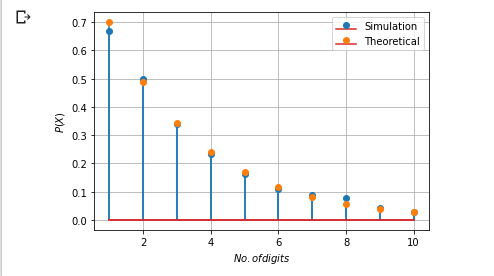
\includegraphics[ width=\columnwidth , height =5cm]{gate_digit.PNG}
\caption{Simulation for tossing a fair coin  }
\label{Fig:1}
\end{figure}
\\\textbf{Download python code from here}\\
\begin{lstlisting}
https://github.com/Swati-Mohanty/AI5002/blob/main/Assignment_7/codes/sim.py
\end{lstlisting}
\textbf{Download latex code from here-}\\
\begin{lstlisting}
https://github.com/Swati-Mohanty/AI5002/blob/main/Assignment_7/codes/assignment7.tex
\end{lstlisting}

\end{document}
